%!TEX root = main.tex

%%%%%%% SECTION %%%%%%%
\section{Modèle évènementiel pour l'intégration du domaine 3D dans les 
EVC}

%\subsection{Introduction}
La méthodologie orientée évènements intègre plusieurs aspects souvent laissés 
de côté dans la littérature concernant le développement les environnements 
virtuels collaboratifs pour la visualisation et la manipulation d'objets 3D. Par 
exemple, elle a l'avantage de proposer un couplage lâche. Dès lors, la réutilisation 
des données produite lors de la collaboration peut facilement être réutiliser pour un 
traitement secondaire comme la sensibilisation aux éléments de l'environnement. 
Le découpage de la modélisation logicielle et l'abstraction qu'elle apporte est aussi 
l'occasion de s'intéresser à la façon dont sont générées les données produites par 
les utilisateurs et la façon dont elles sont affichées. 

L'\gls{EP} occupe, dans le champ de l'informatique, une place centrale dans 
beaucoup de systèmes comme l'énergie, la santé, l'environnement, les transports, 
la finance, les services et l'industrie. L'\gls{EP} réunit des méthodes et des outils 
pour filtrer, transformer, et détecter des motifs dans des évènements, dans le but 
de réagir à des conditions qui changent, généralement liées à des contraintes de 
temps \cite{Chandy2011}. L'\gls{EP} intègre plusieurs fonctionnalités:
\begin{itemize}
	\item Obtenir des données à partir de plusieurs sources en temps (quasi) réel
	\item Agréger et analyser ces données pour détecter des motifs qui indiquent la 
	présence de situation critiques qui nécessitent une réponse
	\item Déterminer la réponse la plus adaptée à ces situations
	\item Surveiller (\textit{monitor}) l'exécution de cette réponse
\end{itemize}

Le panorama d'applications et de technologies proposé par \cite{Hinze2009} 
permet de définir les termes et les interprétations communes à différents 
domaines se basant sur le paradigme de l'\gls{EP}. 



%L'intégration de la partie métier L'un des aspects principaux a été de 
%combiner tous les aspects reliés aux évènements dans le \textit{pipeline} de 
%visualisation et de manipulation d'objets 3D. 


\subsubsection{Constat}

Par nature, une architecture orientée évènements est extrêmement peu couplée et 
hautement distribuée. Le créateur de l'évènement sait seulement que l'évènement 
se produit et n'a aucune idée du traitement l'évènement va subir par 
la suite ou qui cela va concerner. 
C'est pourquoi les architectures orientées évènements sont plus utilisées dans un 
contexte de flux d'information asynchrone. La traçabilité dans ces environnements 
devient alors un enjeu important. Facilitée par l'empreinte laissée par chaque 
évènement, elle n'en demeure pas moins complexe selon l'échelle d'évaluation. A 
l'échelle d'un utilisateur, d'un groupe d'utilisateurs, ou de plusieurs groupes, les 
acteurs restent des entités assez homogènes dans le cadre de la modélisation 3D 
collaborative ce qui simplifie la tâche car on reste dans un cadre et un domaine 
connu.



%Il existe différent types de traitement d'évènement : simple, en continu, 
%complexe. 
%Ils peuvent être utilisés ensemble dans le cadre d'une même application.
%\begin{itemize}
%\item Traitement d'évènement simple. (\textit{simple event processing}). 
%Dans le traitement simple d'évènement, un évènement notable arrive, initiant 
%une 
%cascade d'actions. Le traitement simple d'évènement est généralement utilisé 
%pour 
%orienter un flux temps-réel qui peut prendre un peu de temps, n'entraînant pas de 
%coût sur la partie métier.
%\item Traitement de flux continu d'évènement. (\textit{stream event 
%processing}). 
%\item Traitement d'évènement complexe. (\textit{complex event 
%processing}). 
%
%\end{itemize}

Le choix de baser la gestion des données sur le patron de conception \gls{CQRS} 
combiné à de l'\gls{ES} repose sur le constat suivant : dans un cadre industriel, le 
besoin de traçabilité de l'information est très important pour suivre l'évolution d'un 
projet par exemple. 
Les architectures orientées évènements repose le plus souvent sur 
communication client-serveur pour faciliter la gestion des données dans le 
système distribué. C'est pourquoi l'exploitation du patron de conception 
\gls{CQRS} a originalement été développé avec cette  \gls{CS} qui sont 
toujours connectées (pour récupérer les mises à jour). 
Ce fonctionnement ne permet pas le travail hors ligne.

Côté serveur, le stockage des données est de moins en moins cher, on peut donc 
se permettre de stocker beaucoup de données de manière distante notamment 
grâce au \gls{cloud}\info{definir le cloud}. Le serveur a une puissance de calcul 
plus importante (et surtout ajustable).

Côté client, la puissance de calcul des machines sur lesquelles sont installés les 
navigateurs web évolue rapidement (notamment les appareils mobiles comme les 
\textit{smartphones} et les tablettes). Les navigateurs suivent cette tendance en 
puisant dans ces ressources pour effectuer des traitements similaires à ceux que 
l'on trouve traditionnellement côté serveur et pour proposer des fonctionnalités 
avancées telles que le stockage important de données sur le client (IndexedDB, 
storageAPI), pour l'affichage 3D (WebGL) et pour la communication en \gls{P2P} 
(\gls{WebRTC}). En déportant ainsi la charge que pourrait subir une architecture 
client-serveur côté client, les échangent réseaux sont limités car qui 
sont très coûteux d'un point de vue énergétique pour les appareils mobiles 
\cite{Koskela2015}. De plus, l'utilisation de la bande passante est onéreuse et 
parfois limitée voire inexistante, il est donc nécessaire de tirer parti de tous les 
appareils participant à la collaboration au lieu de tout faire reposer sur le serveur. 
Chaque appareil participant à la collaboration doit être autonome et le plus 
indépendant possible en termes de ressources (données, réseaux, validation 
experte). 


\subsubsection{Contribution}
Pour répondre à cette problématique, nous proposons un modèle pour la 
transmission des données 3D et collaboratives qui permet de  limiter  le nombre 
de requêtes et la taille des données transmises sans perdre la traçabilité de 
celles-ci. L'idée est de profiter de la puissance du client pour créer une 
architecture assurant l'autonomie de l'utilisateur en cas de déconnexion volontaire 
(travaille hors ligne) ou involontaire (coupure). On garantit ainsi à l'utilisateur 
l'utilisation du système avec un historique performant où chaque connexion est 
l'occasion de mettre le système à jour.\improve{en remttre une couche}


\subsection{Modèle général}
La composition de l'architecture s'est effectuée avec en arrière pensée les lignes 
directrices  énoncées plus haut\info{ref section} \cite{Xhafa2010}. 
Utiliser une architecture orientée évènements pour faire de la modélisation 3D peut 
sembler non nécessaire. Cependant lorsqu'on s'intéresse aux apports que cela 
peut générer pour tous les métiers engagés (utilisateurs, développeurs, analystes 
métier) on peut se demander pourquoi cela n'a pas été plus mis en avant 
auparavant. \improve{qu'est ce que ça fait la}La sensibilisation à l'historique des 
données et aux interactions 
inter-utilisateurs est partagée par les utilisateurs et les analystes métier. Quand à 
la sensibilisation à la distribution des données elles est une composante 
importante pour les utilisateurs et les développeurs. Concernant les premiers, cela 
garantit une certaine autonomie dans la création. Pour les seconds, la répartition 
de la charge permet de profiter du potentiel computationnel de toutes les parties 
prenantes du réseau. 

Dans 3DEvent, le langage partagé se réfère au domaine de la manipulation 
d'objets 3D mais aussi au domaine de la collaboration. Par exemple le terme de 
maillage peut se référer à la fois au maillage géométrique ou bien au maillage de 
l'architecture réseau, d'où l'importance de définir les différents contextes en amont. 
Notons que le contexte de l'application peut faire varier les frontières d'un 
domaine. Le modèle issu du domaine défini permet de mettre en valeur les 
aspects métiers liés à l'application.



Le patron \glsreset{ES}\gls{ES} permet de capturer tous les changements d'état 
d'une application sous la forme d'une séquence d'évènements. 
Ces évènements sont conservés dans un journal d'évènements et peuvent être 
rejoués pour retrouver l'état de l'application. 
Les évènements représentent des faits immuables qui sont 
seulement ajoutés au journal les un après les autres, ce qui permet des taux de 
transaction élevés et une réplication efficace (cf Section 
\ref{sec:es}). Dans 3DEvent, plusieurs composants d'\gls{ES} sont étendues selon 
les applications :

\begin{description}
	\item[Acteur] Un acteur consomme des évènements à partir d'un journal 
	d'évènements et produit des évènements pour le même journal d'évènements. 
	L'état interne dérivé à partir des évènements consommés est un modèle 
	d'écriture 
	en mémoire (\textit{in-memory}) et contribue à la partie commande (C) du 
	CQRS\info{reference à la section}.
	\item[Vue] Une vue est un acteur qui ne fait que consommer des évènements à 
	partir du journal d'évènements. L'état interne dérivé à partir des évènements 
	consommés est un modèle de lecture en mémoire et contribue à la partie 
	requête (Q) du CQRS\info{reference à la section}.
	\item[Producteur] Un producteur est un acteur qui produit des évènements à 
	partir 
	du journal d'évènements pour mettre à jour la base de données. L'état interne 
	dérivé 
	à partir des évènements consommés est un modèle de lecture en mémoire et 
	contribue à la partie requête (Q) du CQRS\info{reference à la section}.
	\item[Processeur] Un processeur est un acteur qui consomme des évènements 
	à 
	partir d'un journal d'évènements et produit les évènements traités pour un autre 
	journal d'évènements. Les processeurs peuvent être utilisés pour connecter les 
	journaux d'évènement au traitement des évènements.\info{reference à la 
	section}.
	
\end{description}

%\subsubsection{Collaboration évènementielle}

Les évènements produits par un des composants présentée ci-dessus
peuvent être consommés par d'autres de ces abstractions s'ils partagent un 
journal d'évènements local ou distribué. 

Un \textbf{journal d'évènements} peut fonctionner sur un seul site ou être répliqué 
sur plusieurs sites. 
Le site est considéré comme une zone disponible qui accepte 
l'écriture d'un journal d'évènements local même s'il est partitionné sur plusieurs 
sites. Les journaux d'évènements locaux situés sur plusieurs sites peuvent être 
connectés par le biais d'un journal d'évènements dit \og repliqué\fg{} qui a pour 
responsabilité de préserver l'ordre causal des évènements.\improve{dessin des 
journaux}

Les sites peuvent être situés à des endroits géographiquement distincts ou sur 
des nœuds à l'intérieur d'une même grappe (\textit{cluster}) ou encore être sur le 
même nœud mais traités séparément selon les \improve{c'est quoi}zones 
disponibles nécessaires au fonctionnement de l'application. 
Les Acteurs et les Processeurs écrivent cependant toujours sur leur journal 
d'évènements local. 
Les composants peuvent soit collaborer sur un journal d'évènements local sur le 
même site, ou bien au travers d'un journal répliqué sur différents sites.

Il est important de différencier le journal d'évènements de la base de données 
(côté serveur) ; la base de données peut ne contenir qu'une partie du journal. 
Une base de données peut également être considérée comme un élément 
complémentaire au journal d'évènements, cependant et bien que parfois 
confondus, ils restent bien distincts conceptuellement.

Le journal d'évènements commun est la base des échanges pour communiquer 
par le biais d'évènements de collaboration. Ce type d'architecture se retrouve dans 
différents cas d'utilisation :
\improve{est ce que cette section est nécessaire?}
\begin{itemize}
	\item \textit{Processus métier distribués.} Les acteurs de différents types 
	utilisent des évènements pour communiquer et parvenir à résoudre un problème 
	commun. Bien qu'ils jouent des rôles différents dans le processus métier, ils 
	réagissent à la réception d'évènements (\textit{reactive programming}) en 
	mettant à jour l'état de l'application et en produisant de nouveaux évènements. 
	Cette forme de collaboration est appelée collaboration dirigée par les 
	évènements.\improve{ref}
	\item\textit{Réplication d'état d'Acteur.} Les acteurs de même type consomment 
	les évènements de chacun pour répliquer l'état interne avec une cohérence 
	causale. Dans 3DEvent, les opérations concurrentes sont autorisées dans 
	l'environnement pour mettre à jour l'état des acteurs répliqués et permettre la 
	résolution interactive de conflit en cas de mises à jour concurrentes et 
	conflictuelles. \improve{miuex 
	expliquer}
	\item \textit{Agrégation d'évènement.} Les vues et les producteurs agrègent des 
	évènements à partir d'autres composants pour générer des vues spécifiques à 
	l'application.
	La collaboration évènementielle apporte de la fiabilité dans la gestion des 
	données dans un système distribué. Par exemple, si un processus distribué 
	échoue à cause d'un problème sur une partie du réseau, le système reprend 
	automatiquement dès les répliques sont à jour.
\end{itemize}

%\paragraph{Bus d'évènement}
Les composants souscrivent à leur journal d'évènements en s'accrochant au 
\textbf{bus d'évènements}.
Les évènements nouveaux sont poussés vers les souscripteurs, 
ce qui leur permet de mettre à jour l'état de l'application avec une latence 
minimale. 
Un évènement écrit à un endroit est publié de manière fiable aux souscripteurs sur 
ce site et aux souscripteurs des sites distants. 
Par conséquent, les composants qui échangent par le biais d'un 
journal d'évènements répliqué communiquent via un bus qui préserve l'ordre causal 
des évènements de manière durable et tolérant au partitionnement. De ce fait, les 
services sur les partitions du réseau inter-sites (lien entre les sites) peuvent 
continuer d'écrire des évènements localement. La livraison des évènements sur 
les sites distants reprend automatiquement lorsque les partitions sont à jour.


Le journal d'évènements répliqué localement et fournit un ordre total des 
évènements stockés et appartient à un site. 
Le site est une zone de disponibilité qui héberge un ou plusieurs 
journal d'évènements. Les évènements d'un journal d'évènements sont 
répliqués de manière asynchrone sur les autres des journaux d'évènements 
des sites distants. 
Afin de lier des journaux d'évènements (localisés sur différents sites) à un journal 
d'évènements répliqué, les 
journaux d'évènements locaux doivent être accessibles à partir des points 
d'entrées de réplication. De plus, ces points d'entrée doivent être 
connectés entre eux afin de créer un réseau de réplications. 
Un journal d'évènements répliqué est représenté par un journal d'évènements local 
sur chacun des sites participants.

\info{point d'entrée = network bridge}

Les points d'entrée permettent de gérer un ou plusieurs journaux d'évènements. 
Ces journaux sont identifiés pour permettre à la réplication de ne s'intéresser 
qu'aux journaux de même identifiant. 
Les journaux avec différents identifiants sont ainsi isolés les uns des autres et 
leur distribution peut donc varier selon les sites.

Les journaux répliqués fournissent l'ordre causal des évènements stockés : l'ordre 
de stockage est le même sur tous les sites, ce qui veut dire que les 
consommateurs qui lisent les évènements du journal local vont toujours voir les 
effets avant leurs causes.




\subsection{Mécanisme de gestion de version}
3DEvent intègre une procédure de gestion de version dans l'\gls{EventStore} afin 
de gérer au mieux la cohérence des données. 
Chaque gestion de commande (Figure \ref{fig:gestionCommande}) entraîne la 
génération d'un ou plusieurs évènements. Ces évènements sont considérés 
comme \og soumis\fg{} (\textit{uncomitted}) mais pas encore <<~publiés~>> 
(\textit{comitted}).  Pour qu'ils le deviennent, l'agrégat concerné par ces 
évènements doit produire une nouvelle version sans être en conflit avec la 
précédente. En passant la version attendue $v_a$ au gestionnaire de conflit, on 
est à même de la comparer avec la version courante $v_c$. Il existe deux cas où 
un conflit est levé~: 
\begin{enumerate}[label=\alph*)]
	\item \label{i:vi} La version $v_a$ correspond à la valeur d'initialisation
	\item \label{i:vdiff} La version $v_a$ est différente de la version $v_c$
\end{enumerate}
Dans \ref{i:vi}, on s'assure qu'après une action la version initiale de l'agrégat ne 
peut être la même. Cet item peut sembler évident mais il est important de le noter 
car il dépend entièrement la valeur initiale choisie pour les agrégats du 
\gls{framework} (on peut commencer à n'importe quelle valeur -- -1, 0\ldots).



\subsection{Cohérence Éventuelle en CQRS}

La \gls{CE}, ou \textit{eventual consistency} en anglais, propose dans un système 
distribué contenant plusieurs répliques d'avoir une coordination lâche entre ces 
répliques. Cela apporte de nombreux avantages en termes de disponibilité, 
tolérance aux fautes et sécu rité des données et évite l'intégration de protocoles 2 
phase commit ou de protocoles Paxos (consensus) complexifiant les échanges. 
La\gls{CE} introduit l'idée que toutes les répliques se réconcilient au bout d'un 
moment (\textit{forward progression}) pour avoir le même état final. Si le caractère 
vicié d'une information est détecté, le système doit le \og réparer\fg{} pour obtenir 
le bon état. 

L'ordonnancement des évènements durant les mises à jour reste identique lorsque
les évènements sont rejoués par la suite car l'ordre est issu de l'\gls{ES} est 
déterminée par l'ordonnancement des évènements stockés 
localement. Au sein d'une réplique, tous les composants \gls{CQRS} respectent 
cet ordonnancement. L’ordre de stockage des évènements répliqués sur des sites 
distincts est cohérent à cause de l'ordre causal : les évènements liés 
causalement ont le même ordre sur tous les sites alors que les évènements 
concurrents peuvent avoir un ordre différent. Cette propriété est important pour 
obtenir une cohérence causale (forte) dans une application qui respecte le 
théorème \gls{CAP}.

%Linéaire (strong consistency)
%one version replace another -- one parent and one children in the sequence
%each version is immutable 
%each version has an identity
%each new version is a replacement of the previous (earlier)
%directed acyclic graph (eventual consistency)
%each version may have one or more parent
%each parent may have one or more parent
%each parent may have children with different parents
%each version is immutable
%each version has an identity
%
%each version may be viewed as one of many replacement version for its parents
%
%version are immutable and (should) have immutable names


%\begin{algorithm}[caption="titi"]
%	
%    saveEvents(itemId:string, events:EventMessage[], expectedVersion:number) 
%{\\
%    	var eventDescriptors:EventDescriptor[] = 
%this.eventDescriptorsByAggregate[itemId];\\
%    	if (!eventDescriptors) {\\
%    		eventDescriptors = this.eventDescriptorsByAggregate[itemId] = [];\\
%    	} else if (eventDescriptors.length > 0 \&\& 
%eventDescriptors[eventDescriptors.length\\ - 1].version != expectedVersion \&\& 
%expectedVersion != -1) {\\
%    	throw new Error("ConcurrencyException");\\
%    }
%    var i = expectedVersion;\\
%    events.forEach((event:EventMessage) => {\\
%    	i++;\\
%    	event.version = i;\\
%    	var eventDescriptor = {id: event.AggregateId(), version: i, eventData: 
%event};\\
%    	eventDescriptors.push(eventDescriptor);\\
%    	this.\_publisher.publish(event);\\
%    	this.\_network.publishEvent(event);\\
%    });
%}
%\end{algorithm}
\subsection{Potentielles applications et autres utilisations}
La conception et l'implémentation d'une plateforme comme 3DEvent qui est 
asynchrone, distribuée et orientée évènements  (notamment la persistance) peut 
être appliquée à différents champs.
\begin{description}
	\item[GIT-like app] Les solutions pour faire de la gestion de version, comme 
	MeshGit~\cite{Denning2013} par exemple qui fait du
	\textit{diff and merge} de maillages polygonaux pour des données 3D, 
	sont rarement implémentées (a fortiori en 
	temps-réel) sur des plateformes web à cause du coût et de la complexité que 
	cela peut apporter dans des architectures traditionnelles. 3DEvent peut 
	reconstruire n'importe quel état antérieur grâce à son architecture orientée 
	évènements et indiquer les différences entre deux états.
	
	\item[Scenarii et \textit{path recording}] Pour des jeux sérieux, les graphistes 
	3D ou des études d'ergonomie, cette fonctionnalité est particulièrement 
	pertinente. Le \gls{framework} peut proposer une comparaison entre deux traces 
	laissées par un ou plusieurs utilisateurs. Dans le cas où les utilisateurs ont la 
	même tâche à réaliser, il est facile de faire la différence entre deux réalisations 
	pour comparer, analyser et montrer les résultats	pour des raisons 
	pédagogiques ou pour relever des habitudes (de travail) par exemple. Dans 
	l'exemple du jeu sérieux, on peut comparer la trace utilisateur à la trace experte 
	et permettre de rejouer le même scénario plusieurs fois facilement pour 
	observer l'évolution. Ce type de fonctionnalité est intrinsèque à 3DEvent. 
	
	\item[Traçage utilisateur et \textit{crowdsouring}] 3DEvent peut se révéler être 
	un bon outil pour enregistrer la trace d'un utilisateur lorsqu'il navigue dans la 
	scène. Si on choisit d'enregistrer le chemin de la caméra et les actions 
	utilisateur comme des évènements que l'on considère comme des informations 
	"issues de la foule" (\textit{crowdsouring}). En utilisant un processus 
	d'apprentissage, il est possible de proposer de meilleurs chemins, repérer des 
	points d'intérêt, ou même proposer des résumés de scène générés à partir des 
	traces des collaborateurs (que s'est-il passé depuis la dernière connexion du 
	collaborateur X ?).
	\item[Audit et monitoring de données 3D] L'\gls{ES} fournit un mécanisme 
	d'audit intégré qui assure la cohérence des données transactionnelles. Utiliser 
	ce mécanisme pour faire un audit ou surveiller en temps réel l'activité de 
	l'application peut fournir une meilleure compréhension du travail d'équipe ainsi 
	que l'évolution de la conception. Cela peut permettre de repérer (avec du 
	\gls{CEP}) et corriger certaines fonctionnalités afin d'améliorer l'ergonomie de 
	l'application. Par exemple, si un évènement est anormalement représenté dans 
	le journal des évènements, on va pouvoir lever une alerte facilement.
\end{description}
\begin{figure}[htb]
	\centering
	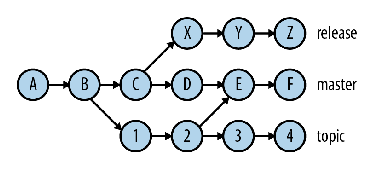
\includegraphics[width=0.3\columnwidth]{gitgraph}
	\caption{Exemple d'arbre de commits Git}
	\label{fig:git}
\end{figure}
\subsection{Bilan}